\newcommand{\bonhommetriste}{
\begin{tikzpicture}[scale=0.2]
	\draw[fill=lightgray] (0, 0) ellipse (1cm and 1cm);
	\draw[fill=blue!50!white] (-0.5, 0.5) ellipse (0.2cm and 0.2cm);
	\draw[fill=blue!50!white] (0.5, 0.5) ellipse (0.2cm and 0.2cm);
	\draw[red, line width=0.5mm] (-0.5, -0.5) edge[bend left=30] (0.5, -0.5);
	\end{tikzpicture}}

\newcommand{\bonhommejoyeux}{
\begin{tikzpicture}[scale=0.2]
	\draw[fill=yellow!50!orange!30!white] (0, 0) ellipse (1cm and 1cm);
	\draw[fill=blue!50!white] (-0.5, 0.5) ellipse (0.2cm and 0.2cm);
	\draw[fill=blue!50!white] (0.5, 0.5) ellipse (0.2cm and 0.2cm);
	\draw[red, line width=0.5mm] (-0.5, -0.5) edge[bend right=30] (0.5, -0.5);
	\end{tikzpicture}}


\newcommand{\photo}[2]{\begin{tabular}{c}\includegraphics[height=1.6cm]{#1} \\[-1mm] {\tiny #2}\end{tabular}}

\newcommand{\tinyphoto}[2]{\begin{tabular}{c}\includegraphics[height=1.2cm]{#1} \\[-1mm] {\footnotesize #2}\end{tabular}}
\newcommand{\photounknown}[1]{\begin{tabular}{c}
\includegraphics[height=1.2cm]{images/Unknown-person.png} \\[-1mm] {\tiny #1}\end{tabular}}






%%%% SETS %%%%%%%%%%%%%%%%%%%%
\newcommand{\union}{\cup}
\newcommand{\Union}{\bigcup}
\newcommand{\bigunion}{\bigcup}
\newcommand{\disjointunion}{\sqcup}
\newcommand{\compose}{\circ}
\newcommand{\compl}[1]{{\overline{{#1}}}}

\newcommand{\inter}{\cap}
\newcommand{\intersection}{\inter}


\newcommand{\Inter}{\bigcap}
\newcommand{\biginter}{\bigcap}
\newcommand{\bigintersection}{\bigcap}

\newcommand{\bigtimes}{\prod}

\newcommand{\infinity}{\infty}
\newcommand{\card}[1]{{\emph{card}(#1)}}
\newcommand{\partiede}[1]{\mathcal P({#1})}

\newcommand{\privede}{\setminus}

\newcommand{\vide}{\emptyset}

\newcommand{\inclu}{\subseteq}
\newcommand{\suchthat}{\mid}
\newcommand{\converse}{^{-1}}



\newcommand{\eqdefine}{=^{\text{def}}}
\newcommand{\eqdef}{\eqdefine}

%%%%% LOGICS %%%%%%%%%%%%%%%%%%%%%%%%
\newcommand{\bigand}{\bigwedge}
\newcommand{\lbigand}{\bigand}
\newcommand{\lAnd}{\bigand}
\newcommand{\bigor}{\bigvee}
\newcommand{\lbigor}{\bigor}
\newcommand{\true}{\top}
\newcommand{\false}{\bot}
\newcommand{\limply}{\Rightarrow}
\newcommand{\logimply}{\limply}
\newcommand{\imp}{\limply}
\newcommand{\imply}{\limply}

\newcommand{\bottom}{\bot}
\newcommand{\lequiv}{\leftrightarrow}


\renewcommand{\phi}{\varphi}

\newcommand{\atmset}{\ensuremath{\mathit{Prop}}\xspace}
\newcommand{\ATM}{\ensuremath{\mathit{Prop}}\xspace}
\newcommand{\valuation}{V}

\newcommand{\subformulasset}[1]{SF(#1)}

\newcommand{\thereisaproof}{\vdash}

\newcommand{\formulalength}[1]{|#1|}


\newcommand{\lbox}{\square}
\newcommand{\logbox}{\lbox}

\newcommand{\ldiamond}{\Diamond}
\newcommand{\tuple}[1]{\langle #1 \rangle}

\newcommand{\frameF}{\mathcal{F}}

\newcommand{\modelM}{\mathcal{M}}
\newcommand{\modelW}{\mathcal{W}}

\newcommand{\classC}{\ensuremath{\mathcal{C}}\xspace}

\newcommand{\logfusion}{\oplus}
\newcommand{\logicfusion}{\logfusion}

\newcommand{\lboxarg}[1]{[#1]}
\newcommand{\logboxarg}[1]{\lboxarg{#1}}

\newcommand{\logdiamarg}[1]{\langle #1 \rangle}
\newcommand{\ldiaarg}[1]{\logdiamarg{#1}}
\newcommand{\ldiamarg}[1]{\logdiamarg{#1}}

%\newcommand{\lknow}[1]{K_{#1}}
%\newcommand{\lknowpos}[1]{\hat K_{#1}}
\newcommand{\lknow}[1]{\Box_{#1}}
\newcommand{\lknowpos}[1]{\Diamond_{#1}}

\newcommand{\possknw}{\lknowpos}

\newcommand{\ldiadiaarg}[1]{\langle \langle #1\rangle \rangle}
\newcommand{\latl}[1]{\ldiadiaarg{#1}}
\newcommand{\logdiaboxarg}[1]{\langle[#1]\rangle}
\newcommand{\ldiamboxarg}[1]{\logdiaboxarg{#1}}
\newcommand{\ldiaboxarg}[1]{\logdiaboxarg{#1}}
\newcommand{\logiclanguage}[1]{{\ensuremath{\mathcal{L}_{#1}}\xspace}}

\newcommand{\lognext}{X}
\newcommand{\loginthefuture}{F}
\newcommand{\lnext}{\lognext}
\newcommand{\linthefuture}{\loginthefuture}

\newcommand{\loguntil}{U}
\newcommand{\luntil}{\loguntil}

\newcommand{\agtset}{\ensuremath{\textit{Agt}}\xspace}
\newcommand{\actset}{\ensuremath{\textit{ACT}}\xspace}
\newcommand{\AGT}{\ensuremath{\textit{Agt}}\xspace}

\newcommand{\lposempty}{\ldiaarg{\emptyset}}

\newcommand{\worldsset}{W}
\newcommand{\aworld}{w}
\newcommand{\aworldb}{u}

\newcommand{\grammaris}{\hspace{2mm}::=\hspace{2mm}}
\newcommand{\grammarseparation}{\hspace{2mm}\mid\hspace{2mm}}

















%% SPECIFIC SETS %%%%%%%%%%%%%%%%%%%%%%%%%%

\newcommand{\inN}{\in \mathbb{N}}
\newcommand{\ZnZ}[1]{ \mathbb{Z}/ { {#1} \mathbb{Z} } }

\newcommand{\setN}{\mathbb{N}}
\newcommand{\Nset}{\setN}
\newcommand{\ensN}{\setN}

\newcommand{\setR}{\mathbb{R}}
\newcommand{\Rset}{\setR}
\newcommand{\ensR}{\setR}

\newcommand{\setQ}{\mathbb{Q}}
\newcommand{\Qset}{\setQ}
\newcommand{\ensQ}{\setQ}

\newcommand{\setW}{\mathbb{W}}
\newcommand{\Wset}{\setW}
\newcommand{\ensW}{\setW}



%% LOGIC NAMES %%%%%%%%%%%%%%%

%&latex
\newcommand{\logicCSTIT}{\textsf{CSTIT}\xspace}
\newcommand{\logicXCSTIT}{\textsf{XCSTIT}\xspace}
\newcommand{\logicSTIT}{\textsf{STIT}\xspace}
\newcommand{\logicCL}{\textsf{CL}\xspace}
\newcommand{\logicATL}{\textsf{ATL}\xspace}
\newcommand{\logicATLstar}{\ensuremath{\textsf{ATL}^*}\xspace}
\newcommand{\logicCTL}{\textsf{CTL}\xspace}
\newcommand{\logicCTLstar}{\ensuremath{\textsf{CTL}^*}\xspace}
\newcommand{\logicInt}{\textsf{Int}\xspace}

\newcommand{\logicATLbox}[1]{\langle \langle #1 \rangle \rangle}
\newcommand{\logicSfive}{\textsf{S5}\xspace}
\newcommand{\logicSfour}{\textsf{S4}\xspace}
\newcommand{\logicSfourdottree}{\textsf{S4.3}\xspace}
\newcommand{\logicK}{\textsf{K}\xspace}
\newcommand{\logicPDL}{\textsf{PDL}\xspace}
\newcommand{\logicPTL}{\textsf{PTL}\xspace}
\newcommand{\logicLTL}{\textsf{LTL}\xspace}
\newcommand{\logicAlt}{\textsf{Alt}\xspace}

\newcommand{\logicindividualSTIT}{ind\logicSTIT}
\newcommand{\logicindSTITbox}[1]{\lboxarg{#1}}
\newcommand{\logicindSTITposbox}{\lbox}
\newcommand{\logiclog}[1]{\textsf{log}(#1)}

\newcommand{\momentsset}{M}
\newcommand{\historiesset}{H}
\newcommand{\amoment}{m}
\newcommand{\ahistory}{h}

\newcommand{\cstit}[1]{[#1]}











%%%%%% ENVIRONMENTS %%%%%%%%%%%%%%%%%%%%%%%%%%%
%
%\newtheorem{theorem}{Theorem}
%\newtheorem{conjecture}{Conjecture}
\newtheorem{remark}{Remark}
%\newtheorem{proposition}{Proposition}
%\newtheorem{question}{Question}
%\newtheorem{property}{Property}
%\newtheorem{notation}{Notation}
%\newtheorem{definitionThm}{Definition}
%\newtheorem{example}{Example}
%\newtheorem{lemma}{Lemma}
%\newtheorem{corollary}{Corollary}
%\newtheorem{proofThm}{Proof}

%\newenvironment{proof}{
%  \textsc{Proof.}
%    {~\\}
%    \normalfont
%    \indent
%  }{$\blacksquare$}

\newcommand{\proofof}[1]{\fbox{#1}}

%\newenvironment{definition}[1][]{%
%\begin{definitionThm}[#1]~\\%
%\normalfont%
%}
%{
%\end{definitionThm}%
%}





%%%%%% ALGORITHMS %%%%%%%%%%%%%%%%%%%%%%%%%%%%%%%%

\newcommand{\algofunction}{\textbf{function }}
\newcommand{\algofunctionul}{\textbf{function }}
\newcommand{\algoprocedure}{\textbf{procedure }}
\newcommand{\recursive}{\textbf{recursive }}
\newcommand{\algoendfunction}{\textbf{endFunction }}
\newcommand{\algoendprocedure}{\textbf{endProcedure }}
\newcommand{\algofor}{\textbf{for }}
\newcommand{\algodo}{\textbf{do }}
\newcommand{\algoendfor}{\textbf{endFor }}


\definecolor{algocommentbackgroundcolor}{rgb}{1,1,0.5}

\newcommand{\algocomment}[1]{\colorbox{algocommentbackgroundcolor}{\begin{minipage}{\textwidth}\small{#1}\end{minipage}}}

\newcommand{\algocommentoneline}[1]{\colorbox{algocommentbackgroundcolor}{\small{#1}}}
\newcommand{\algowhile}{\textbf{while }}
\newcommand{\algoendwhile}{\textbf{endWhile }}

\newcommand{\algoif}{\textbf{if }}
\newcommand{\algothen}{\textbf{then }}
\newcommand{\algoelse}{\textbf{else }}
\newcommand{\algoendif}{\textbf{endIf }}

\newcommand{\algomatch}{\textbf{match }}
\newcommand{\algoendmatch}{\textbf{endMatch }}

\newcommand{\algocase}{\textbf{case }}


\newcommand{\return}{\textbf{return }}
\newcommand{\algoreturn}{\textbf{return }}
\newcommand{\algochoose}{\textbf{choose }}
\newcommand{\algochooseexists}{\textbf{choose ($\exists$)}}
\newcommand{\algochooseforall}{\textbf{choose ($\forall$)}}
\newcommand{\algocall}{\textbf{call }}

\newcommand{\algoaccept}{\textbf{accept }}
\newcommand{\algoreject}{\textbf{reject }}

\newlength{\algoindentlongueur}
\setlength{\algoindentlongueur}{1cm}
\newcommand{\algoindent}{\hspace*{\algoindentlongueur}}

\newlength{\algoindentavantvrulelongueur}
\setlength{\algoindentavantvrulelongueur}{0.2cm}
\newcommand{\algoindentavantvrule}{\hspace*{\algoindentavantvrulelongueur}}

\newcommand{\functionname}[1]{\underline{#1}}


\newcommand{\algocommentaire}[1]{\emph{commentaire : #1}}
\newlength{\dummy}


\newsavebox{\frameminipageboiteavecunnomsuperlongdesortequonnepuissepaslereutiliser}
\newenvironment{frameminipage}[2][c]{%
\begin{lrbox}{\frameminipageboiteavecunnomsuperlongdesortequonnepuissepaslereutiliser}%
\begin{minipage}[#1]{#2}%
} {%
\end{minipage}%
\end{lrbox}%
\framebox{\usebox{\frameminipageboiteavecunnomsuperlongdesortequonnepuissepaslereutiliser}}%
}


\newenvironment{algo} {
  \begin{frameminipage}{\linewidth}
} {
  \end{frameminipage}
}

\newenvironment{algobloc}{\setlength{\dummy}{\linewidth}\addtolength{\dummy}{- \algoindentlongueur}\addtolength{\dummy}{- \algoindentavantvrulelongueur}\algoindentavantvrule\vrule\algoindent\begin{minipage}{\dummy}}{\end{minipage}}


\newenvironment{algoblocfunction}[1]
{\algofunction #1 \\  \begin{algobloc}}
{\end{algobloc} \algoendfunction}

\newenvironment{algoblocif}[1]
{\algoif #1 \algothen \\  \begin{algobloc}}
{\end{algobloc} \algoendif}

\newenvironment{algoblocfor}[1]
{\algofor #1 \algodo \\  \begin{algobloc}}
{\end{algobloc} \algoendfor}


\newenvironment{algoblocmatch}[1]
{\algomatch #1 \algodo \\  \begin{algobloc}}
{\end{algobloc} \algoendmatch}

\newenvironment{algobloccase}[1]
{\algocase #1 : \\  \begin{algobloc}}
{\end{algobloc}}









%%%%%%%%%%%%% INDEX %%%%%%%%%%%%%%%%%%%%%

\newcommand{\indexprint}[1]{#1\index{#1}}
\newcommand{\indexemph}[1]{\emph{#1}\index{#1}}










\newcommand{\agent}{a}
\newcommand{\agenta}{a}
\newcommand{\agentb}{b}
\newcommand{\agentc}{c}

\newcommand{\cartearg}[1]{\tikz{\node[minimum height=5mm, inner sep=1mm, fill=white, draw] {#1};}}
\newcommand{\cartea}{\cartearg{$\clubsuit$}}
\newcommand{\carteb}{\cartearg{\textcolor{red}{$\Diamondblack$}}}

\newcommand{\cartec}{\cartearg{\textcolor{red}{$\varheartsuit$}}}

\newcommand{\mondecartes}[3]{\begin{tabular}{c}
		
\includegraphics[scale=0.06]{images/possibleworld.png} \\[-18mm]
		\begin{tabular}{C{1mm}C{1mm}C{1mm}}
			\agenta&\agentb&\agentc\\[-4mm]
			#1 & #2 & #3
		\end{tabular}

	\end{tabular}}

\newcommand{\mondereelcartes}[3]{\begin{tabular}{c}
		
\includegraphics[scale=0.06]{images/realworld.png} \\[-18mm]
		\begin{tabular}{C{1mm}C{1mm}C{1mm}}
			\agenta&\agentb&\agentc\\[-4mm]
			#1 & #2 & #3
		\end{tabular}

	\end{tabular}}


\newcommand{\enfantsalegd}{\begin{tikzpicture}[scale=0.3]
	\draw[fill=yellow!20] (0, 0) ellipse (1cm and 1cm);
	\draw[fill=blue!20] (0.3, 0.1) ellipse (.25cm and .25cm);
	\draw[fill=black] (0.4, 0.1) ellipse (.15cm and .15cm);
	\draw[red, line width=0.5mm] (0.2,-.3) edge[out=-90, in=180] (0.7, -0.7);
	\node at (0.4, 0.7) {
\includegraphics[scale=0.03]{images/tache.png}};
	\node at (-0.5, 0) {\tiny a};
	\end{tikzpicture}}

\newcommand{\enfantpropregd}{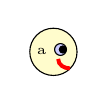
\begin{tikzpicture}[scale=0.3]
	\draw[fill=yellow!20] (0, 0) ellipse (1cm and 1cm);
	\draw[fill=blue!20] (0.3, 0.1) ellipse (.25cm and .25cm);
	\draw[fill=black] (0.4, 0.1) ellipse (.15cm and .15cm);
	\draw[red, line width=0.5mm] (0.2,-.3) edge[out=-90, in=180] (0.7, -0.7);
	\node at (-0.5, 0) {\tiny a};
%	\node at (0.4, 0.7) {\includegraphics[scale=0.03]{images/tache.png}};
	\end{tikzpicture}}


	\newcommand{\enfantsaledg}{\begin{tikzpicture}[scale=0.3]
\draw[fill=yellow!20] (0, 0) ellipse (1cm and 1cm);
\draw[fill=blue!20] (-0.3, 0.1) ellipse (.25cm and .25cm);
\draw[fill=black] (-0.4, 0.1) ellipse (.15cm and .15cm);
\draw[red, line width=0.5mm] (-0.2,-.3) edge[out=-90, in=0] (-0.7, -0.7);
		\node at (-0.4, 0.7) {
\includegraphics[scale=0.03]{images/tache.png}};
		\node at (0.5, 0) {\tiny b};
		\end{tikzpicture}}

	\newcommand{\enfantpropredg}{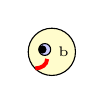
\begin{tikzpicture}[scale=0.3]
\draw[fill=yellow!20] (0, 0) ellipse (1cm and 1cm);
\draw[fill=blue!20] (-0.3, 0.1) ellipse (.25cm and .25cm);
\draw[fill=black] (-0.4, 0.1) ellipse (.15cm and .15cm);
\draw[red, line width=0.5mm] (-0.2,-.3) edge[out=-90, in=0] (-0.7, -0.7);
\node at (0.5, 0) {\tiny b};
		%	\node at (0.4, 0.7) {\includegraphics[scale=0.03]{images/tache.png}};
		\end{tikzpicture}}


\newcommand{\mondereelenfantssales}[2]{\begin{tabular}{c}
	%	
\includegraphics[scale=0.08]{images/realworld.png} \\[-18mm]
			#1  #2 %\\[3mm]
		%	~
	\end{tabular}}




\newcommand{\mondepossibleconsecutivenumbers}[2]{\begin{tabular}{cc}
		%	
\includegraphics[scale=0.08]{images/realworld.png} \\[-18mm]
		#1 & \hspace{-2mm}#2 \\
		\enfantpropregd &\hspace{-2mm} \enfantpropredg %\\[3mm]
		%	~
	\end{tabular}}

\newcommand{\mondepossibleenfantssales}[2]{\begin{tabular}{c}
	%	
\includegraphics[scale=0.08]{images/possibleworld.png} \\[-18mm]
		#1  #2 % \\[3mm]
	%	~
	\end{tabular}}




\newcommand{\mondereel}{
\includegraphics[scale=0.08]{images/realworld.png}}
\newcommand{\mondepossible}{
\includegraphics[scale=0.08]{images/possibleworld.png}}
\newcommand{\mondepossiblepetit}{
\includegraphics[scale=0.04]{images/possibleworld.png}}
\newcommand{\mondepossiblepetitdeux}{
\includegraphics[scale=0.04]{images/possibleworld2.png}}



\definecolor{citebibliocolor}{rgb}{0,0,0.5}
\newcommand{\citebiblio}[1]{
\includegraphics[scale=0.3]{images/paper.jpg}~ [\textcolor{citebibliocolor}{\footnotesize{#1}}]}




\definecolor{FORMULE_COLOR}{rgb}{0.9,0.9,0.9}
\newcommand\formule[1]{{\colorbox{FORMULE_COLOR}{\ensuremath{#1}}}}








	\newcommand{\propositionaestsale}{\propositiontxt{$a$ is dirty}}
	\newcommand{\propositionbestsale}{\propositiontxt{$b$ is dirty}}

	\newcommand{\muddyA}{\propositionaestsale}
	\newcommand{\muddyB}{\propositionbestsale}


	%\newcommand{\question}[1]{
	%	\tikz{\node[fill=green!50!white, inner sep=0.2mm, rounded corners] {\raisebox{-1mm}{
\includegraphics[width=5mm]{images/help.png}} \begin{minipage}{8.5cm}\footnotesize #1\end{minipage}};}}

	\newcommand{\question}[1]{}



	\newtheorem{proposition}{Proposition}


\definecolor{PROP_COLOR}{rgb}{0.8,0.8,0.8} 
\newcommand\propositionmath[1]{\colorbox{PROP_COLOR}{\ensuremath{#1}}}
\newcommand\propositiontxt[1]{\text{\colorbox{PROP_COLOR}{\footnotesize #1}}}
\newcommand\propositiontxtsmall[1]{\text{\colorbox{PROP_COLOR}{\small #1}}}


% epistemic models
\newcommand{\epsmodel}{\mathcal M}
\newcommand\relworldsa{R_a}
\newcommand\valworlds V
\newcommand\world w
\newcommand{\setworlds}{W}
\newcommand{\initialmodelrelation}{R}
\newcommand{\initialmodelrelationagent}[1]{R_{#1}}
\newcommand{\valuationfunction}{V}
\newcommand{\epsmodelfull}{\epsmodel=(\setworlds,\{\relworldsa\}_{a\in\agtset},\valworlds)}


% event models
\newcommand\eventmodel{\mathcal E}
\newcommand{\setevents}{E}

\newcommand{\releventsa}{\mathbb R_a}
\NewDocumentCommand{\relevents}{O{a}}{\rightarrow_{#1}}
\NewDocumentCommand{\equivevents}{O{}}{\mathbb R}%{\sim_{#1}}
\NewDocumentCommand{\equivwords}{O{}}{\mathbb R}%{\sim_{#1}}
\newcommand\event e
\newcommand\eventmodelfull{\eventmodel=(\setevents,\{\releventsa\}_{a\in\agtset},\pre, \post)}


\newcommand\ie{\emph{i.e.}\xspace}
\newcommand\eg{\emph{e.g.}\xspace}



\newcommand{\langEL}{\logiclanguage K}

\newcommand\languageEL{\langEL}

\newcommand{\langDEL}{\logiclanguage {DEL}}

\newcommand{\Ka}{\lknow a}

\newcommand{\egdef}{:=}












\newcommand{\putcamerawithoutcone}[3]{
	\node[camera] at (#1, #2)  {};
	\node at (#1, #2+0.4)  {\ensuremath{#3}};
}

\definecolor {conevisionboundarycolor}{rgb}{0.8,0.4,0.07} 

\tikzstyle{camera} = [draw, circle, fill=black, inner sep=0.5mm]


\tikzstyle{conevisionboundary} = [conevisionboundarycolor]


%\putcamerawithdistanceangle x y angle angleopening distanceofvision name
\newcommand{\putcamerawithdistanceangle}[6]{
	\draw[conevisionboundary] (#1, #2) -- +(#3-#4/2:#5);
	\draw[conevisionboundary] (#1, #2) -- +(#3+#4/2:#5);
	\draw[fill=yellow!40, opacity=0.5,draw=none] (#1, #2) -- +(#3-#4/2:#5)  -- +(#3+#4/2:#5);
	\node at (#1, #2+0.5)  {\ensuremath{#6}};
	\node[camera] at (#1, #2)  {};
}


\newcommand{\putcamerawithdistanceanglered}[6]{
	\draw[conevisionboundary] (#1, #2) -- +(#3-#4/2:#5);
	\draw[conevisionboundary] (#1, #2) -- +(#3+#4/2:#5);
	\draw[fill=yellow!40, opacity=0.5,draw=none] (#1, #2) -- +(#3-#4/2:#5)  -- +(#3+#4/2:#5);
	\node[red] at (#1, #2+0.5)  {\ensuremath{#6}};
	\node[camera, red] at (#1, #2)  {};
}

\tikzstyle{agentin2dworld} = [fill=white]

\tikzstyle{world} = [circle, draw]
\tikzstyle{transition} = [->, line width=1mm]


\pgfdeclareradialshading{glow}{\pgfpoint{0cm}{0cm}}{
	color(0mm)=(white);
	color(3mm)=(white);
	color(7mm)=(black);
	color(10mm)=(black)
}

\begin{tikzfadingfrompicture}[name=glow fading]
	\shade [shading=glow] (0,0) circle (1);
\end{tikzfadingfrompicture}

\tikzfading[name=fade out, 
inner color=transparent!0,
outer color=transparent!100]


\tikzstyle{epistemicmodel} = [
draw=none,
path fading=glow fading,
fill=white,path picture={
	\node[path fading=glow fading] at (path picture bounding box.center){
		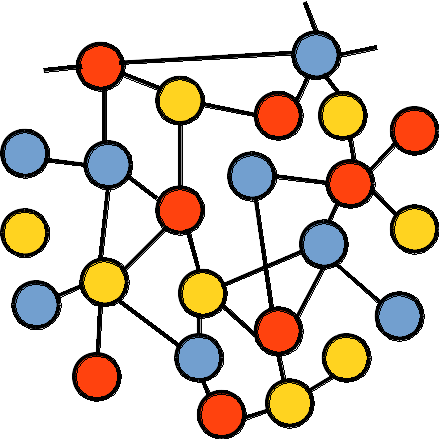
\includegraphics[width=2.5cm]{images/theoreme_de_de_bruijn_erdos_no_transparency.png} };
}]





\newcommand{\queueautomatatransition}[3]{(#1, #2, #3)}



\newcommand{\queueautomatonletterpinpointed}{\letter}
\newcommand{\queueautomatonletterqcq}{\letter'}
\newcommand{\queueautomatonlettera}{\letter_1}
\newcommand{\queueautomatonletterb}{\letter_2}
\newcommand{\queueautomatonletterc}{\letter_3}

\newcommand{\queueautomatonfinalstates}{F}
\newcommand{\debut}{\textit{start}\xspace}
\newcommand{\error}{\textit{error}\xspace}
\newcommand{\push}{{\textsf{push}}} % "push" typographié
\newcommand{\pop}{{\textsf{pop}}} % "pop" typographié
\newcommand{\enqueue}{{\textsf{enqueue}}} % "enqueue" typographié
\newcommand{\dequeue}{{\textsf{dequeue}}} % "dequeue" typographié

\newcommand{\queueautomaton}{\mathcal{A}}
\newcommand{\queueautomatonstates}{S}
\newcommand{\queueautomatonstate}{s}
\newcommand{\queueautomatonstateinitial}{\queueautomatonstate_{ini}}
\newcommand{\queueautomatonwordqueue}{q}


\NewDocumentCommand{\queueautomataconfigurationepistemicmodel}{O{}O{}O{}O{}O{}}{
	\begin{tikzpicture}[xscale=0.9]
	\tikzstyle{innersepsmall} = [inner sep=0.5mm];
	\node[world, innersepsmall, initial left, initial text={}] (q0) at (0, 0) {$#1$};
	
	\ifthenelse{\isempty{#2}}{}
	{\node[world, innersepsmall] (q1) at (1, 0) {$#2$};}
	\ifthenelse{\isempty{#3}}{}
	{\node[world, innersepsmall] (q2) at (2, 0) {$#3$};}
	
	\ifthenelse{\isempty{#4}}{}
	\node[world, innersepsmall] (q3) at (3, 0) {$#4$};
	
	\ifthenelse{\isempty{#5}}{}
	\node[world, innersepsmall] (q4) at (4, 0) {$#5$};
	
	\draw[->] (q0) edge[loop below] (q0);
	
	\ifthenelse{\isempty{#2}}{}
	\draw[->] (q0) edge[] (q1);
	
	\ifthenelse{\isempty{#3}}{}
	\draw[->] (q1) edge[] (q2);
	
	\ifthenelse{\isempty{#4}}{}
	\draw[->] (q2) edge[] (q3);
	
	\ifthenelse{\isempty{#5}}{}
	\draw[->] (q3) edge[] (q4);	
	\end{tikzpicture} 
}





\newcommand{\langPropositional}{\mathcal L_{\atmset}}

\newcommand{\Ereal}{E_{rep}}%{E_{real}}

\newcommand{\planninginstance}{(\modelM, w, \eventmodel, \Ereal, \phi)}

\newcommand{\DELpres}{(\modelM,\modelE)}
\NewDocumentCommand{\update}{O{}}{\modelM \otimes \modelE^{#1}}
\NewDocumentCommand{\DELstruct}{O{*}}{\modelM \modelE^{#1}}
\newcommand{\DELstructfull}{\DELstruct=
	(\traceSet,\relhist, \relhiststar, \{\relM{\agent}\}_{\agent\in\agtset},\valuationfunction)}
\newcommand{\DELstructOnlyKnowledgeAndRelHistfull}{\DELstruct=
	(\traceSet,\relhist, \{\relM{\agent}\}_{\agent\in\agtset},\valuationfunction)}
\newcommand{\DELstructOnlyKnowledgefull}{\DELstruct=
	(\traceSet, \{\relM{\agent}\}_{\agent\in\agtset},\valuationfunction)}

\newcommand{\trace}{h}
\newcommand{\traceSet}{\mathcal H}
\newcommand\ME[1]{\mathcal{ME}^{#1}} % ME calligraphié avec exposant (nom générique de structure DEL si #1 = *)
\newcommand\MEe{\ME{*}} % ME* calligraphié (nom générique de structure DEL)
\newcommand{\relM}[1]{\initialmodelrelationagent{#1}} % symbole pour relation épistémique d'un modèle épistémique

\newcommand{\relhist}{\bm{\rightarrow}} % symbole pour relation épistémique d'un modèle épistémique
\newcommand{\relhiststar}{\relhist^*}


\newcommand{\modelE}{\mathcal{E}}
\newcommand{\relE}[1]{\initialmodelrelationagent{#1}} % symbole pour relation épistémique d'un modèle d'événements 
\newcommand{\propreal}{\texttt{real}}
\newcommand{\reldyn}{\rightarrow}


\newtheorem{notation}{Notation}


\renewcommand{\alert}[1]{\textcolor{blue!80!white}{#1}}

\newcommand{\goalformula}{\phi}

\newcommand\ampoule{
\includegraphics[height=8mm]{images/ampoule.jpg}}

\newcommand{\realworld}{w}
\newcommand{\planlength}{\ell}




\newcommand\eventinfigure{\evenement}
\newcommand\postconditionpfalse{p := \faux}
\newcommand{\postconditiontrivial}{-}



\newcommand{\evenement}[2]{
			\begin{tabular}{l}\mbox{pre}: \ensuremath{#1} \\[-0mm] \mbox{post}:$\begin{array}{ll}
					#2
				\end{array}$
			\end{tabular}
	}
	
	
	
	
	
	
	\newcommand{\evenementpossible}[2]{
		\raisebox{-4.5mm}{\begin{tikzpicture}[inner sep=0mm]
			\node[anchor=west] {\begin{tikzpicture}	[scale=0.4]
				\draw[fill=yellow!50!orange, draw=none] (0, 0) --(1, 0) -- (0.2, -1) -- (0.6,-1) -- (-0.1,-1.8) -- (0.2,-1.8) -- (-1, -3) -- (-0.6,-2) -- (-1,-2) -- (-0.1,-1.2) -- (-0.6,-1.2) -- cycle;
				\end{tikzpicture}
			};
			\node[anchor=west]  {~~~\begin{tabular}{l}\mbox{pre}: #1 \\[-1mm] \mbox{post}: #2
				\end{tabular}};
			\end{tikzpicture}}
		}
		







		\newcommand{\vrai}{\ensuremath{\mathbf{true}}}
		\newcommand{\faux}{\ensuremath{\mathbf{false}}}
		
		%\newcommand{\evenementpossiblejustedessin}{\begin{tikzpicture}	[scale=0.2]
		%	\draw[fill=yellow!50!orange, draw=none] (0, 0) --(1, 0) -- (0.2, -1) -- (0.6,-1) -- (-0.1,-1.8) -- (0.2,-1.8) -- (-1, -3) -- (-0.6,-2) -- (-1,-2) -- (-0.1,-1.2) -- (-0.6,-1.2) -- cycle;
		%	\end{tikzpicture}}
		%\ %newcommand{\evenementpossiblejustedessindeux}{\begin{tikzpicture}	[scale=0.2]
		%	\draw[fill=yellow!50!orange!80!green, draw=none] (0, 0) --(1, 0) -- (0.2, -1) -- (0.6,-1) %%-- (-0.1,-1.8) -- (0.2,-1.8) -- (-1, -3) -- (-0.6,-2) -- (-1,-2) -- (-0.1,-1.2) -- (-0.6,-1.2) -- cycle;
		%	\end{tikzpicture}}
		
		
		\newcommand{\evenementtrivial}{\evenement{\vrai}{-}}
		\newcommand{\evenementpossibleqq}{\evenementpossible {..} {..}}
		
		
		
		
		\newcommand{\propositionrizcasserole}{\propositiontxt{rice in the pot}}
		\newcommand{\propositionpatescasserole}{\propositiontxt{pasta in the pot}}
		\newcommand{\propositionpatespretes}{\propositiontxt{pasta are ready}}
		\newcommand{\propositionrizpret}{\propositiontxt{rice is ready}}
		
		
		
		
		\newcommand{\propositionconsecutivenumber}[2]{\propositiontxt{$#1$'s number is #2}}
		
		
		\newcommand\eventinfigurewithtrivialpostcondition[1]{\evenement{#1}{-}}
		
		
		\tikzstyle{event} = [inner sep=0mm, draw]
\tikzstyle{initialworld} = [initial left, initial text={}]
\tikzstyle{realevent} = [initial left, initial text={}]
\tikzstyle{realabove} = [initial above, initial text={}]
\tikzstyle{realworldarrowfromleft} = [initial left, initial text={}]


\newcommand{\drawloopforaandbup}[1]
{
	\draw (#1)	edge[loop above] node[above] {$a, b$} (#1);
}

\newcommand{\drawloopforaandbleft}[1]
{
	\draw (#1)	edge[loop left, looseness=3] node[left] {$a, b$} (#1);
}

\newcommand{\drawloopforbright}[1]
{
	\draw (#1)	edge[loop right, looseness=3] node[right] {$b$} (#1);
}

\newcommand{\drawloopforaleft}[1]
{
	\draw (#1)	edge[loop left, looseness=3] node[left] {$a$} (#1);
}

\newcommand{\drawloopforbleft}[1]
{
	\draw (#1)	edge[loop left, looseness=3] node[left] {$b$} (#1);
}


\tikzstyle{inEreal} = [fill=blue!20!white]


\newcommand{\epistemicplanninginstancetuple}{(\modelM, \realworld, \eventmodel, \Ereal, \goalformula)}




%\reductiondiagram problem1 problem2 instance1 instance2
\newcommand\reductiondiagram[4]{ \begin{tikzpicture}[remember picture, inner sep=0.2cm]
	\node[draw,fill= gray!10] (p1) {
		\begin{tikzpicture}
		\node [draw,fill= gray!30] (reduction) {reduction};
		\node  [ above right =5mm and 1mm of reduction] (p1label)  {\begin{tabular}{l}#1\end{tabular}};
		\node[right=2mm of reduction] (instanceP2) {#4};
		\node [draw,right=2mm of instanceP2,fill= white] (p2) {\begin{tabular}{l}#2\end{tabular}};
		\draw[->] (reduction) edge (instanceP2);
		\draw[->] (instanceP2) edge (p2);
		\end{tikzpicture}
	};
	
	\node[left=5mm of reduction] (instanceP1) {#3};
	\node[right=5mm of p2] (resultP1) {};
	\draw[->] (instanceP1) -- (reduction);
	\draw[->] (p2) -- (resultP1);
\end{tikzpicture}}


\newcommand{\schemareduction}[4]{
	\begin{center}
		\reductiondiagram{#1}{#2}{#3}{#4}
	\end{center}
}



\newcommand{\grosotimes}{{\huge\textcolor{blue}{$\otimes$}}}
\newcommand{\grosegal}{\textcolor{blue}{\huge=}}

\newcommand{\fadingsouth}[1]{\begin{tikzpicture}
	\node[scope fading=south] {#1};
	\end{tikzpicture}}


\tikzstyle{boite} = [draw, minimum height=1.5cm, minimum width=3cm, fill=white]
\tikzstyle{field} = [blue]
\tikzstyle{myfield} = [blue, fill=blue!20!white]